\section{Results and Discussion}\label{sec:results}
The results presented in this section are divided into the two datasets as described in Section~\ref{sec:exp}. Dataset $A$ are taken from~\cite{lv2021multi} and demonstrate the performance of \AlgName{} on a diversity of problems with different sizes; while dataset $B$ investigates the effect of problem size and error type.

\subsection*{Dataset A}

Table~\ref{tab:results-a} gives the results from 30 runs of \AlgName{} and the base-line co-kriging algorithm on problems $f10$ to $f17$ from~\cite{lv2021multi}, comprising dataset $A$.

\begin{table*}[h!]
\centering
\caption{Results on dataset $A$ comparing the base-line co-kriging algorithm to \AlgName{}. Given are the number of decision variables ($D$), the square of the Pearson correlation coefficient ($r^2$), the best objective obtained, the mean best objective over the full set of runs ($\mu$) and the corresponding standard deviation ($\sigma$).}\label{tab:results-a}
% \begin{adjustbox}{width=\columnwidth}
\begin{tabular}{lrrrrrrrr} \toprule
& & & \multicolumn{3}{c}{Co-kriging} & \multicolumn{3}{c}{\AlgName{}}\\
\cmidrule(lr){4-6} \cmidrule(lr){7-9}
Instance & $D$ & $r^2$ &\multicolumn{1}{c}{best}&\multicolumn{1}{c}{\(\mu\)} & \multicolumn{1}{c}{\(\sigma\)}&\multicolumn{1}{c}{best}& \multicolumn{1}{c}{\(\mu\)}&\multicolumn{1}{c}{\(\sigma\)}\\ \midrule
%
$f10$ & 3 & 0.64 & \best{0} &  \best{2.2960}  &  3.5445  &    \best{0} & 3.9189 &  5.3296\\
$f11$ & 3 & 0.74 &   \best{0.0001} &  0.0110  &  0.0077  &  0.0004 &   \best{0.0098} &  0.0064\\
$f12$ & 4 & 0.79 & -8.1107 &  -3.8007 &  1.3426 &  \best{-9.5783} & \best{-5.8853}  &  1.5123\\
$f13$ & 4 & 0.89 &   0.6290 &  4.9366  &  5.0965  &  \best{0.0519} &   \best{0.3457} &  0.1971\\
$f14$ & 5 & 0.75 &   \best{0.2509} &  \best{0.2583}  &  0.0039  &  0.2522 &   0.2607 &  0.0037\\
$f15$ & 6 & 0.78 & 104.2304 &  1700.28 &  2015.04 & \best{24.6278} & \best{152.9817} &144.6451\\
$f16$ & 8 & 0.82 & \best{7.3904}   &  196.810 &  171.7771&  7.9240 &  \best{75.2898} & 59.3423\\
$f17$ & 8 & 0.79 & -2.5859  &  42.0074 &  153.4414& \best{-3.0161} & \best{-2.8355} & 0.0967\\
%
\bottomrule
\end{tabular}
% \end{adjustbox}
\end{table*}

In this table, it can be seen that \AlgName{} performs as well as, or better than, the base-line co-kriging algorithm, with a few exceptions. For the tests on instances $f11$, $f14$ and $f16$ the base-line co-kriging algorithm was able to find at least one solution that was better than the best solution produced by \AlgName{}, and for the instances $f10$ and $f14$ it produced better solutions on average. In all of these instances, the differences between the algorithms are small, with both performing very similarly; whereas \AlgName{} outperforms the co-kriging by some margin in a lot of the other instances.

This is supported by the convergence plots in Figure~\ref{fig:set-a-conv}. Here, it is clear that when the size of the problem is small, the performance of the two algorithms is very similar, with similar convergence rates; but as the size increases, the both the average performance, and convergence rate, of \AlgName{} over co-kriging improves significantly --- with the most marked improvement being for problem $f17$.

\begin{figure*}[t]
  \centering
  \subfloat[$f11\ (D=3)$\label{fig:f11-conv}]{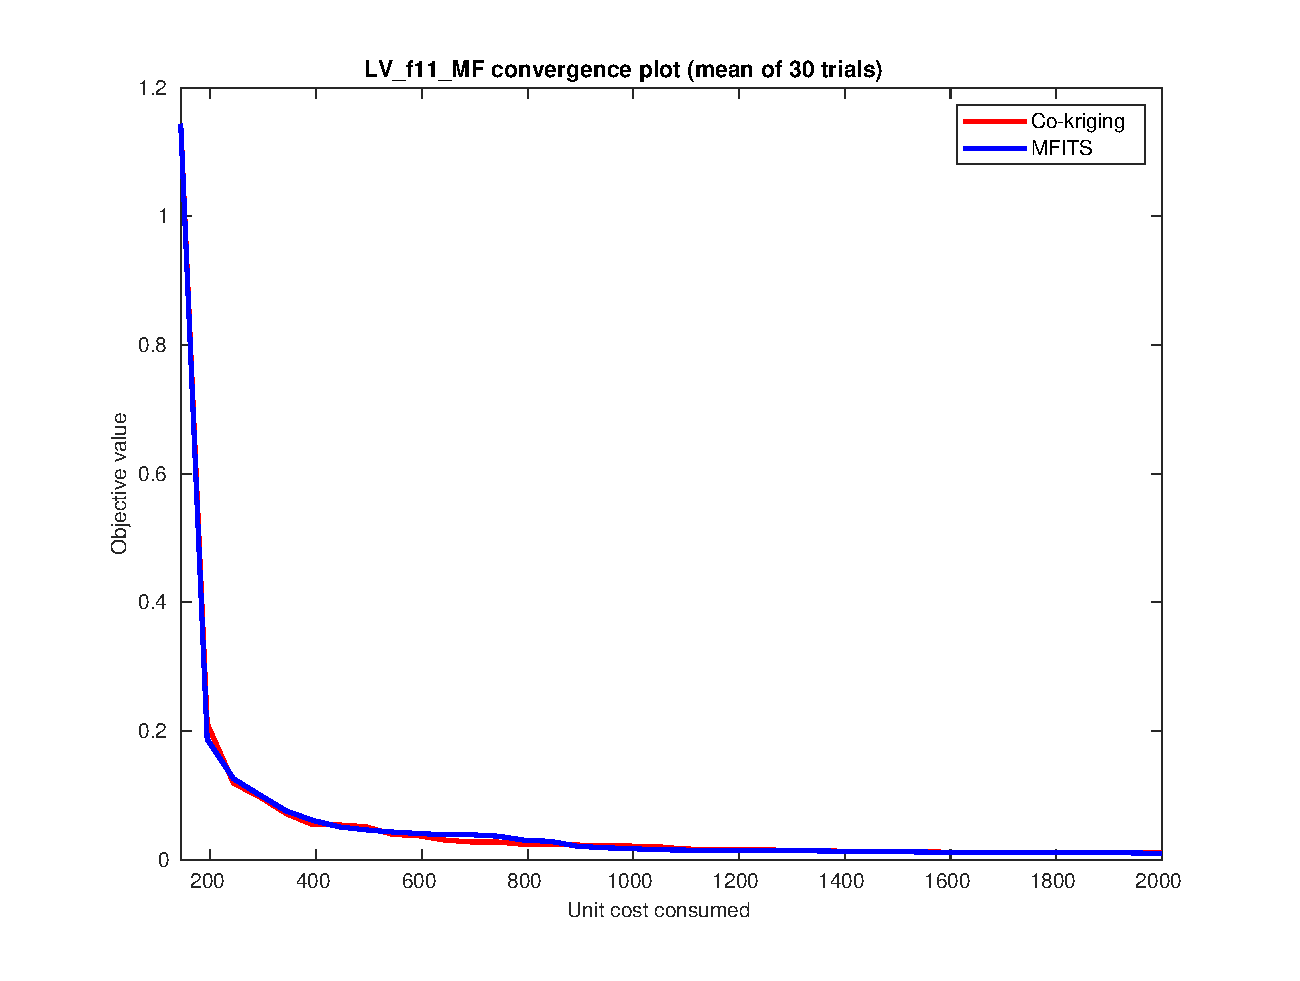
\includegraphics[width = 0.33\textwidth]{img/LV_f11_MF_conv_mean.eps}}
  \subfloat[$f13\ (D=4)$\label{fig:f13-conv}]{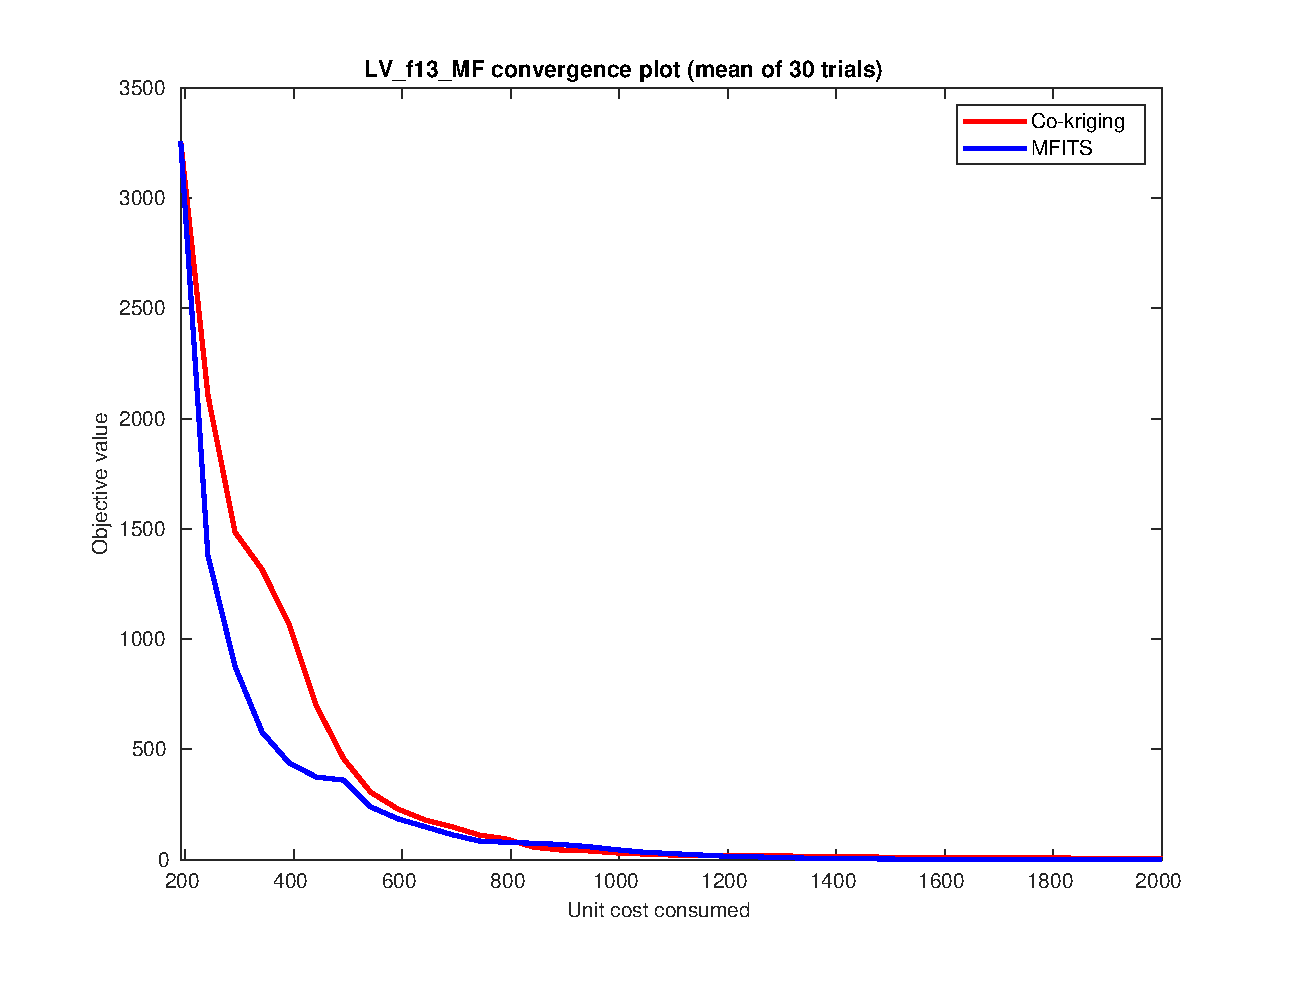
\includegraphics[width = 0.33\textwidth]{img/LV_f13_MF_conv_mean.eps}}
  \subfloat[$f14\ (D=5)$\label{fig:f14-conv}]{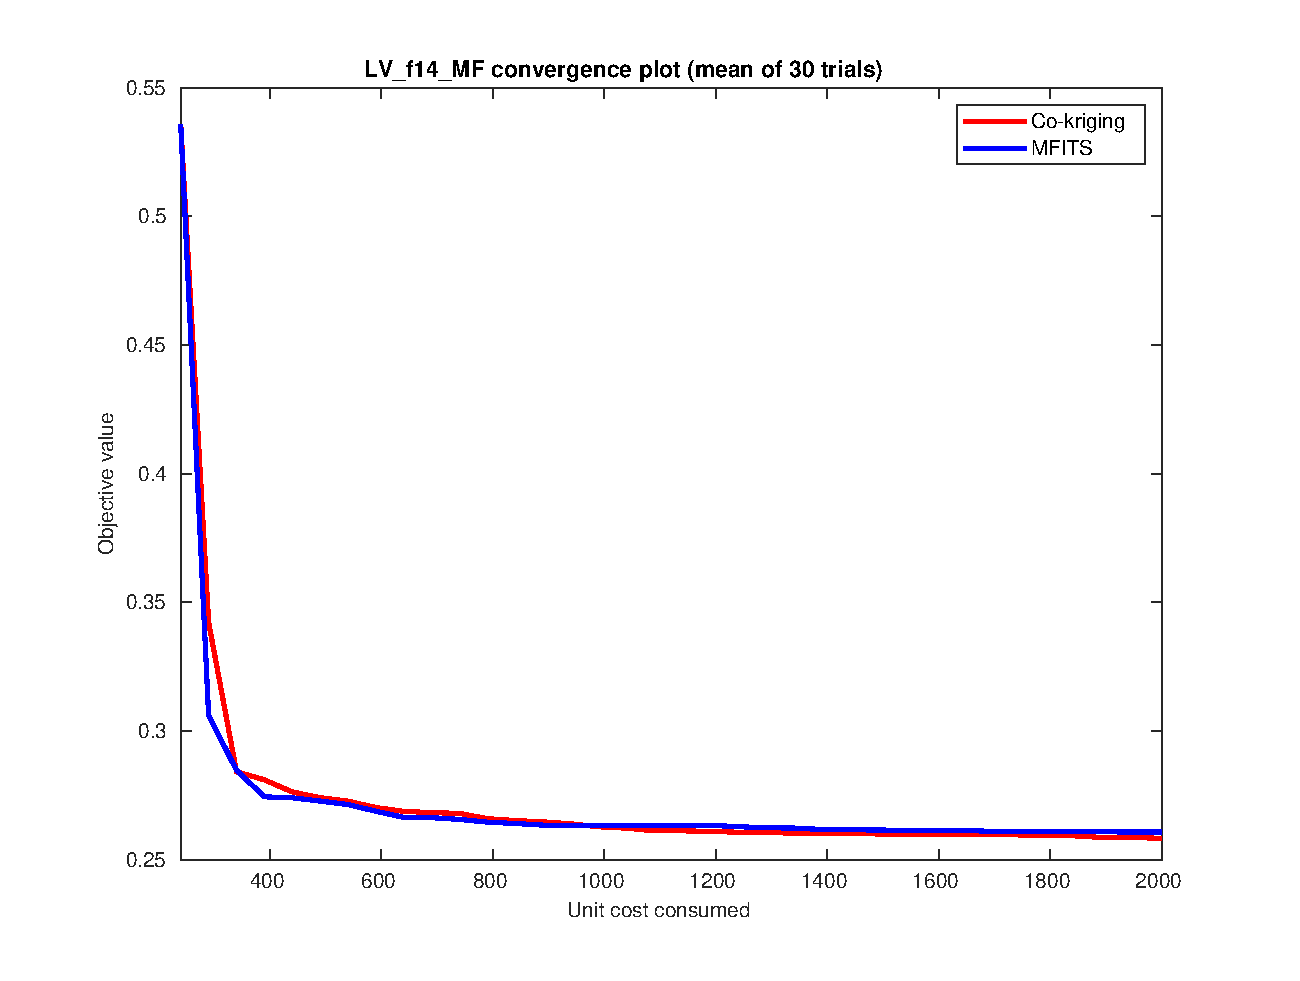
\includegraphics[width = 0.33\textwidth]{img/LV_f14_MF_conv_mean.eps}}\\
  \subfloat[$f15\ (D=6)$\label{fig:f15-conv}]{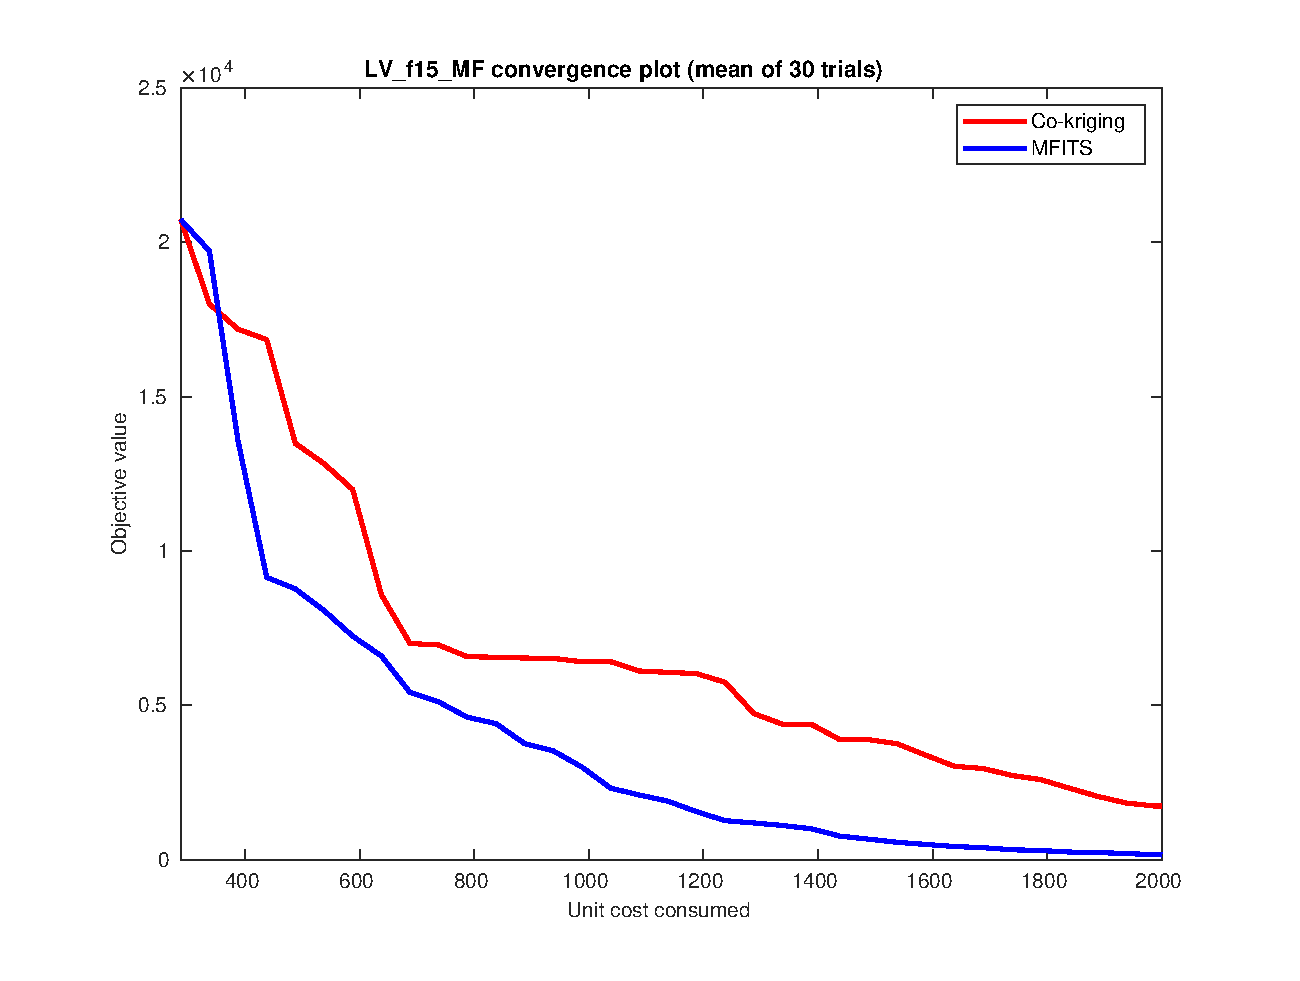
\includegraphics[width = 0.33\textwidth]{img/LV_f15_MF_conv_mean.eps}}
  \subfloat[$f16\ (D=8)$\label{fig:f16-conv}]{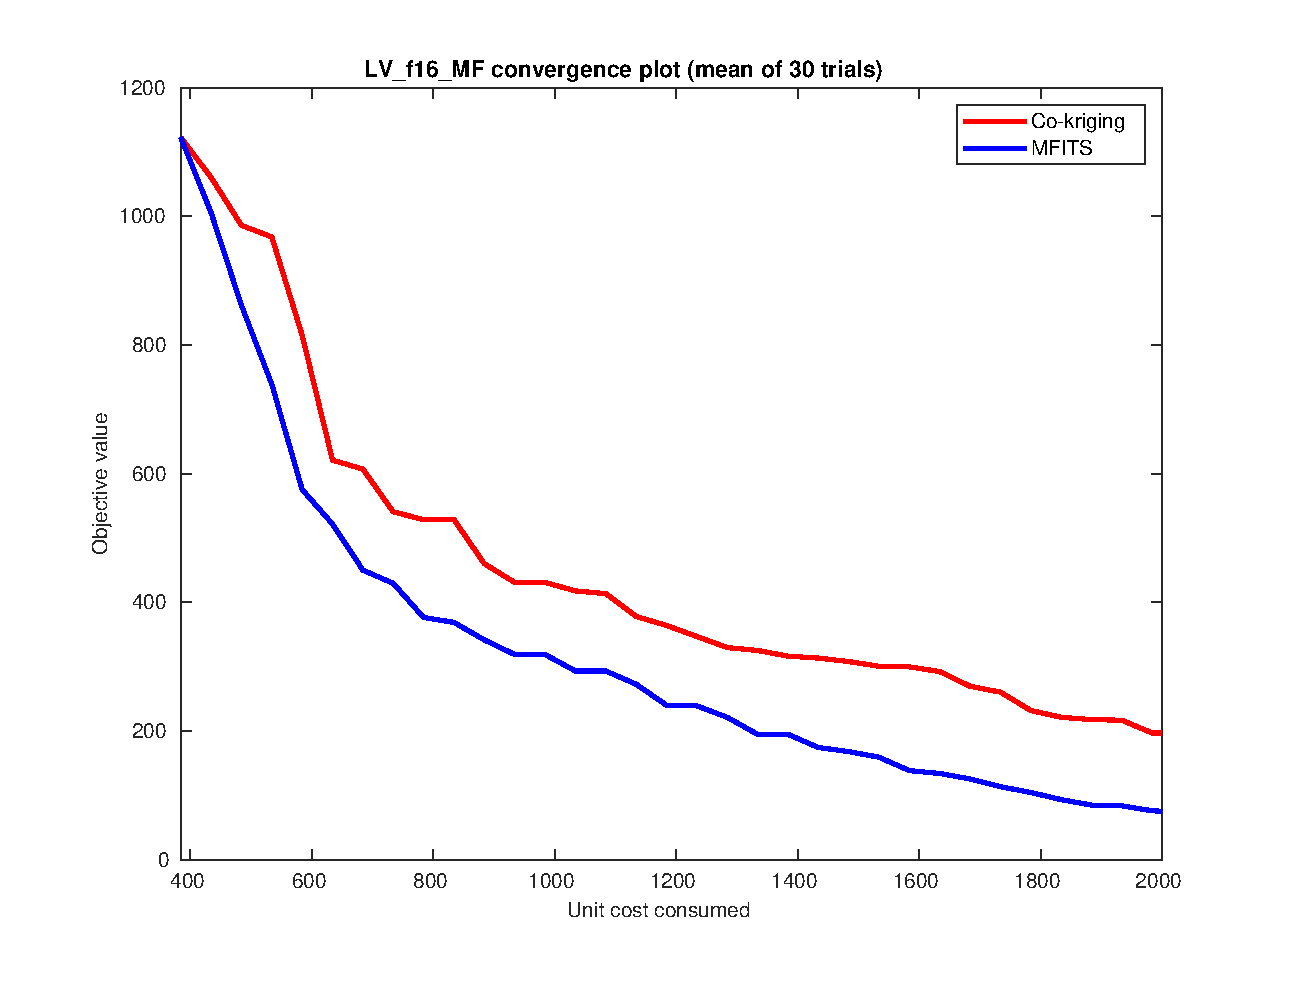
\includegraphics[width = 0.33\textwidth]{img/LV_f16_MF_conv_mean.eps}}
  \subfloat[$f17\ (D=8)$\label{fig:f17-conv}]{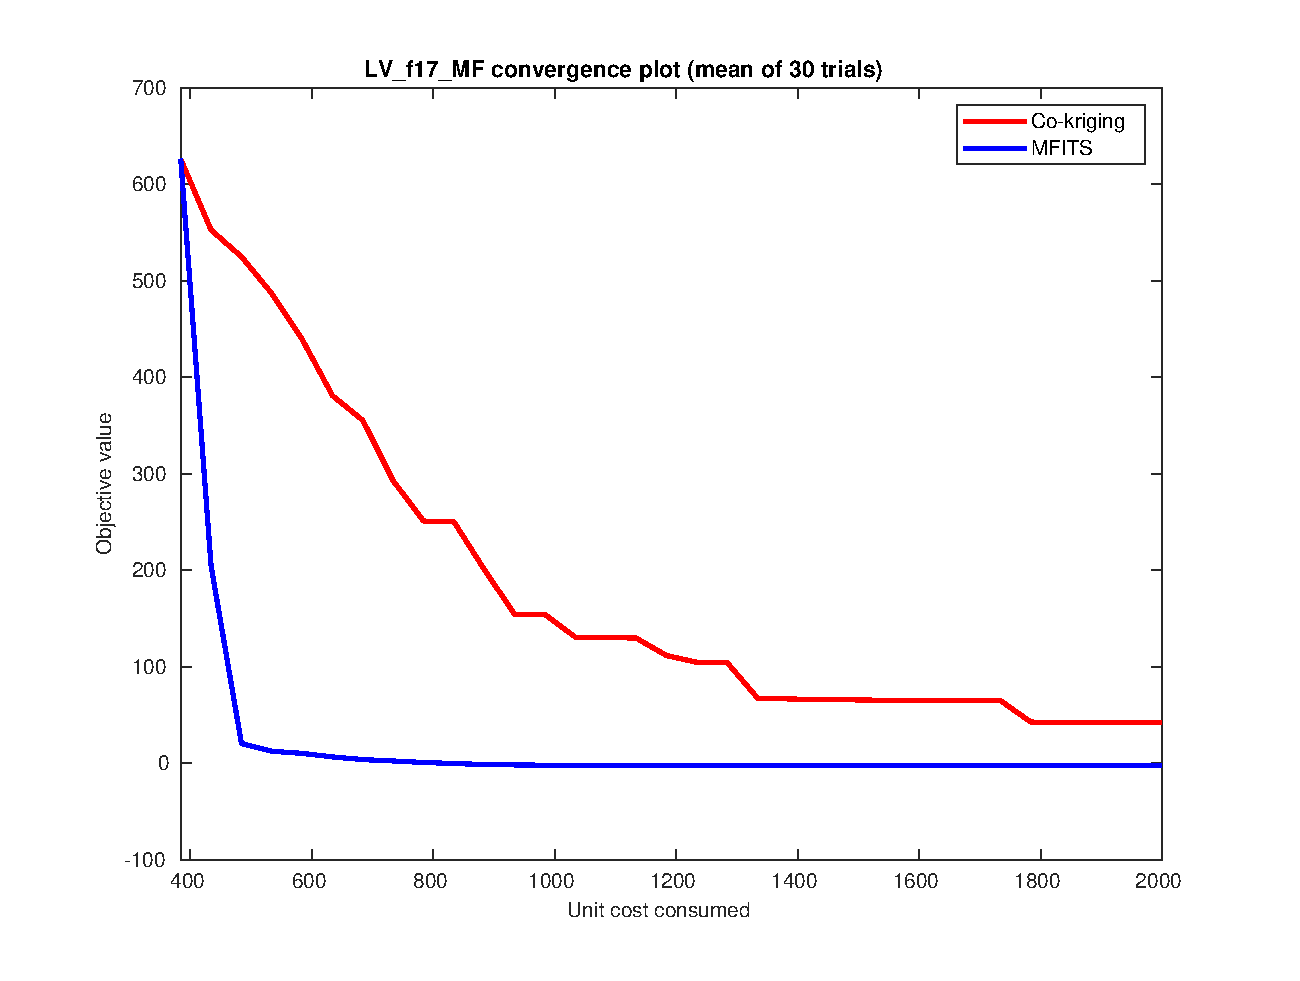
\includegraphics[width = 0.33\textwidth]{img/LV_f17_MF_conv_mean.eps}}
  \caption{Mean convergence plots for problem instances $f11$, $f13$, $f14$, $f15$, $f16$ and $f17$ of dataset $A$, over 30 runs. \angus{will do pgfplots version}} 
    \label{fig:set-a-conv}
\end{figure*}

\subsection*{Dataset B}

The purpose of dataset $B$ was to observe the effect of problem size on the performance of \AlgName{}, and to do so using two different error functions to ensure the results obtained are consistent, and not dependent on the simulation error model used.

\begin{table*}[h!]
\centering
\caption{Results on Griewank and Michalewicz test problems using Wang error functions 2 and 6 (indicated by subscript), comparing the base-line co-kriging algorithm to \AlgName{}. Given are the number of decision variables ($D$), the square of the Pearson correlation coefficient ($r^2$), the best objective obtained, the mean best objective over the full set of runs ($\mu$) and the corresponding standard deviation ($\sigma$).}\label{tab:results-b}
% \begin{adjustbox}{width=\columnwidth}
\begin{tabular}{lrrrrrrrr} \toprule
& & & \multicolumn{3}{c}{Co-kriging} & \multicolumn{3}{c}{\AlgName{}}\\
\cmidrule(lr){4-6} \cmidrule(lr){7-9}
Instance & $D$ & $r^2$ & \multicolumn{1}{c}{best}&\multicolumn{1}{c}{\(\mu\)} & \multicolumn{1}{c}{\(\sigma\)}&\multicolumn{1}{c}{best}& \multicolumn{1}{c}{\(\mu\)}&\multicolumn{1}{c}{\(\sigma\)}\\ \midrule
%
$Griewank_{2}$    & 3 & 0.73 & \best{0} &  \best{0.0018} &  0.0083 & \best{0} &   0.0072 &  0.0137\\
                  & 5 & 0.54 & \best{0} &  0.0535 &  0.0733 & \best{0} &   \best{0.0485} &  0.1055\\%
                  & 8 & 0.37 & \best{0} &  0.6538 &  0.3363 & \best{0} &   \best{0.1864} &  0.2531\\
$Griewank_{6}$    & 3 & 0.74 & \best{0} &  \best{0.0056} &  0.0114 & \best{0} &   0.0104 &  0.0130\\
                  & 5 & 0.76 & \best{0} &  0.0730 &  0.1145 & \best{0} &   \best{0.0361} &  0.0778\\
                  & 8 & 0.76 & \best{0} &  0.4560 &  0.4238 & \best{0} &   \best{0.2089} &  0.3539\\
\midrule  
$Michalewicz_{2}$ & 3 & 0.77 &  -2.7239 & -2.3582 &  0.2587 & \best{-2.7360} &  \best{-2.5305} &  0.1557\\
                  & 5 & 0.73 &  -3.5164 & -2.9470 &  0.2921 & \best{-3.5653} &  \best{-2.9953} &  0.3219\\%
                  & 8 & 0.64 &  -4.1813 & -3.0214 &  0.5671 & \best{-4.2150} &  \best{-3.0818} &  0.7827\\
$Michalewicz_{6}$ & 3 & 0.76 &  -2.7194 & -2.2412 &  0.2978 & \best{-2.7409} &  \best{-2.3142} &  0.2411\\
                  & 5 & 0.83 &  \best{-3.6198} & -2.7140 &  0.3948 & -3.5511 &  \best{-2.9104} &  0.2823\\
                  & 8 & 0.86 &  -3.9978 & -3.1032 &  0.4929 & \best{-4.2922} &  \best{-3.1363} &  0.0909\\
%
\bottomrule
\end{tabular}
% \end{adjustbox}
\end{table*}

The results in Table~\ref{tab:results-b} compare the performance of \AlgName{} and the baseline co-kriging algorithm and are taken over 30 runs on two problem instances from the literature, with varying numbers of decision variables using error functions $e_2$ and $e_6$ as described in~\cite{wang2017generic}.

The table shows that in the majority of instances \AlgName{} outperforms the co-kriging baseline algorithm, with a few exceptions. For the Michaelwicz problem using error function $e_6$ and has been instantiated with five decision variables, the co-kriging base-line algorithm managed to find the best over-all solution, however \AlgName{} still performed better on average. The only time when the co-kriging base-line outperformed \AlgName{} on average was the two smallest instantiations of the Griewank problem. The convergence plots in Figures~\ref{fig:gw23-conv} and~\ref{fig:gw63-conv} show that the difference between the performance of both algorithms for these instances is reasonably negligible. The remaining plots in Figure~\ref{fig:set-b-conv} agree with the results on dataset $A$.

\begin{figure*}[h!]
  \centering
  \subfloat[$Griewank_2\ (D=3)$\label{fig:gw23-conv}]{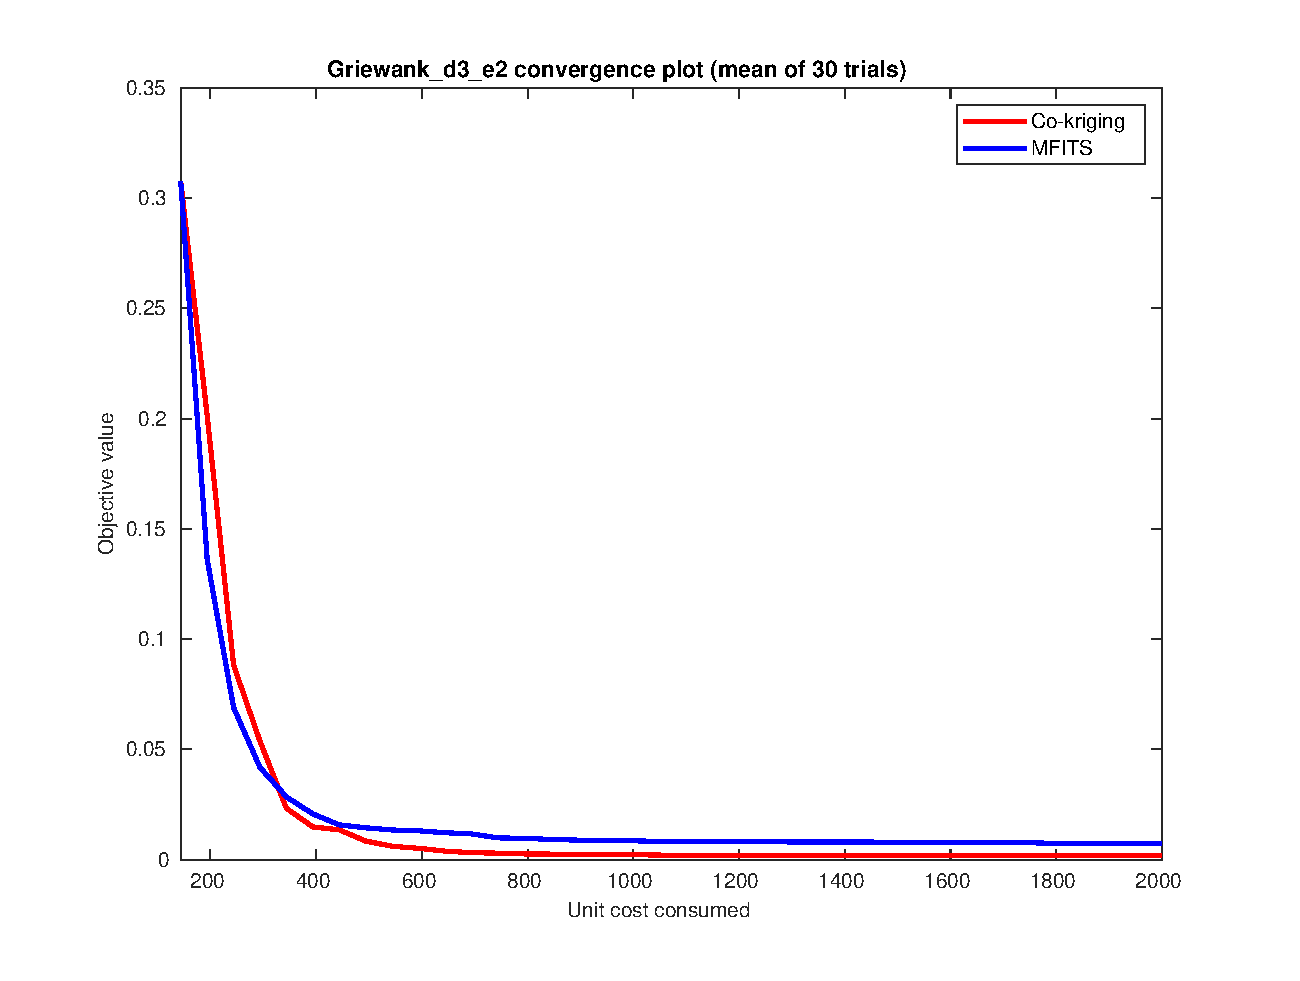
\includegraphics[width = 0.33\textwidth]{img/GW_d3_e2_conv_mean.eps}}
  \subfloat[$Griewank_2\ (D=5)$\label{fig:gw25-conv}]{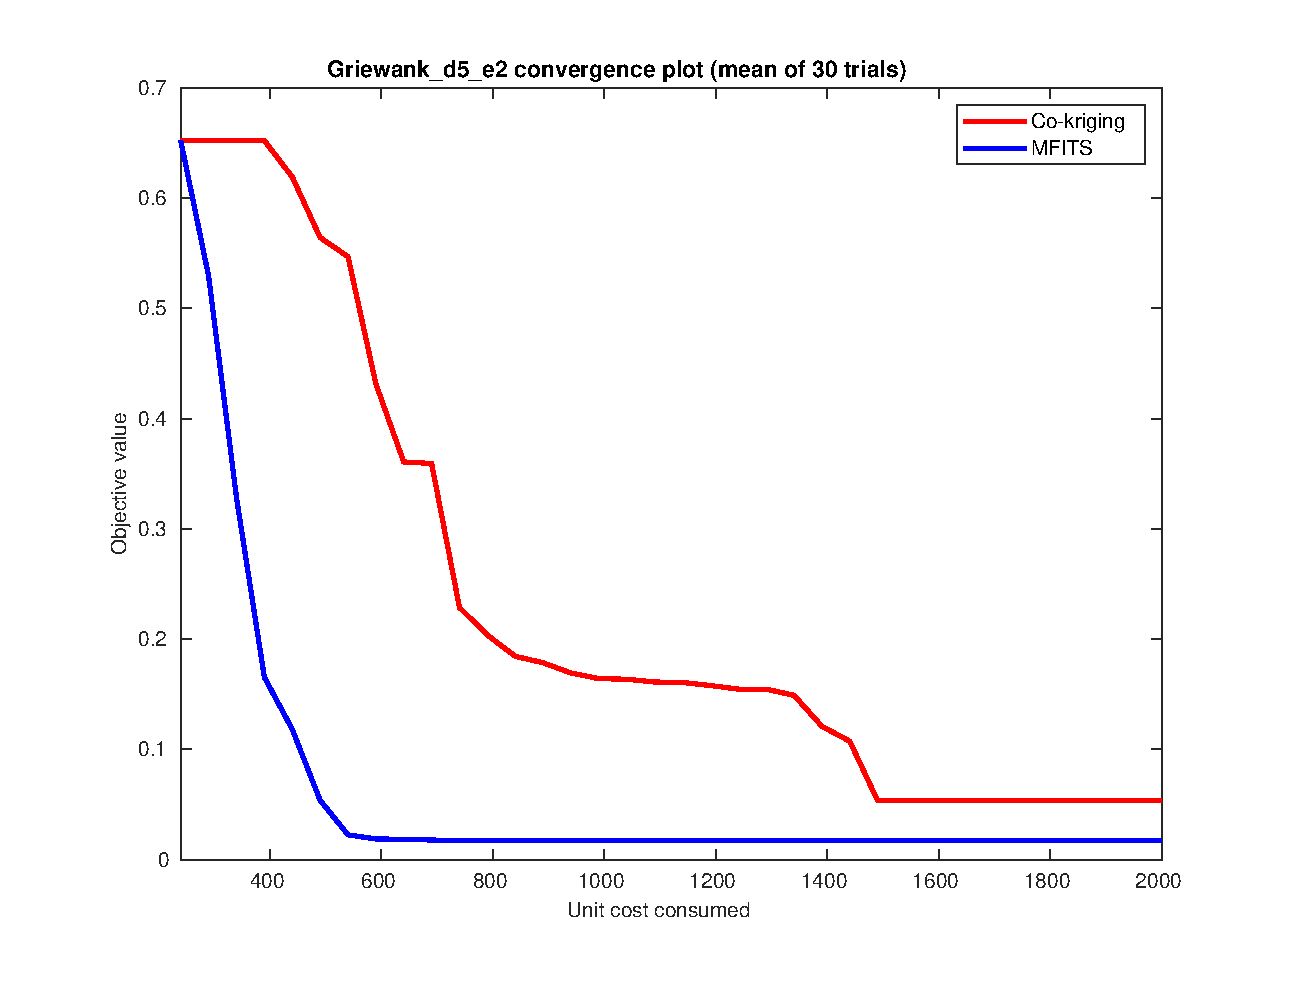
\includegraphics[width = 0.33\textwidth]{img/GW_d5_e2_conv_mean.eps}}
  \subfloat[$Griewank_2\ (D=8)$\label{fig:gw28-conv}]{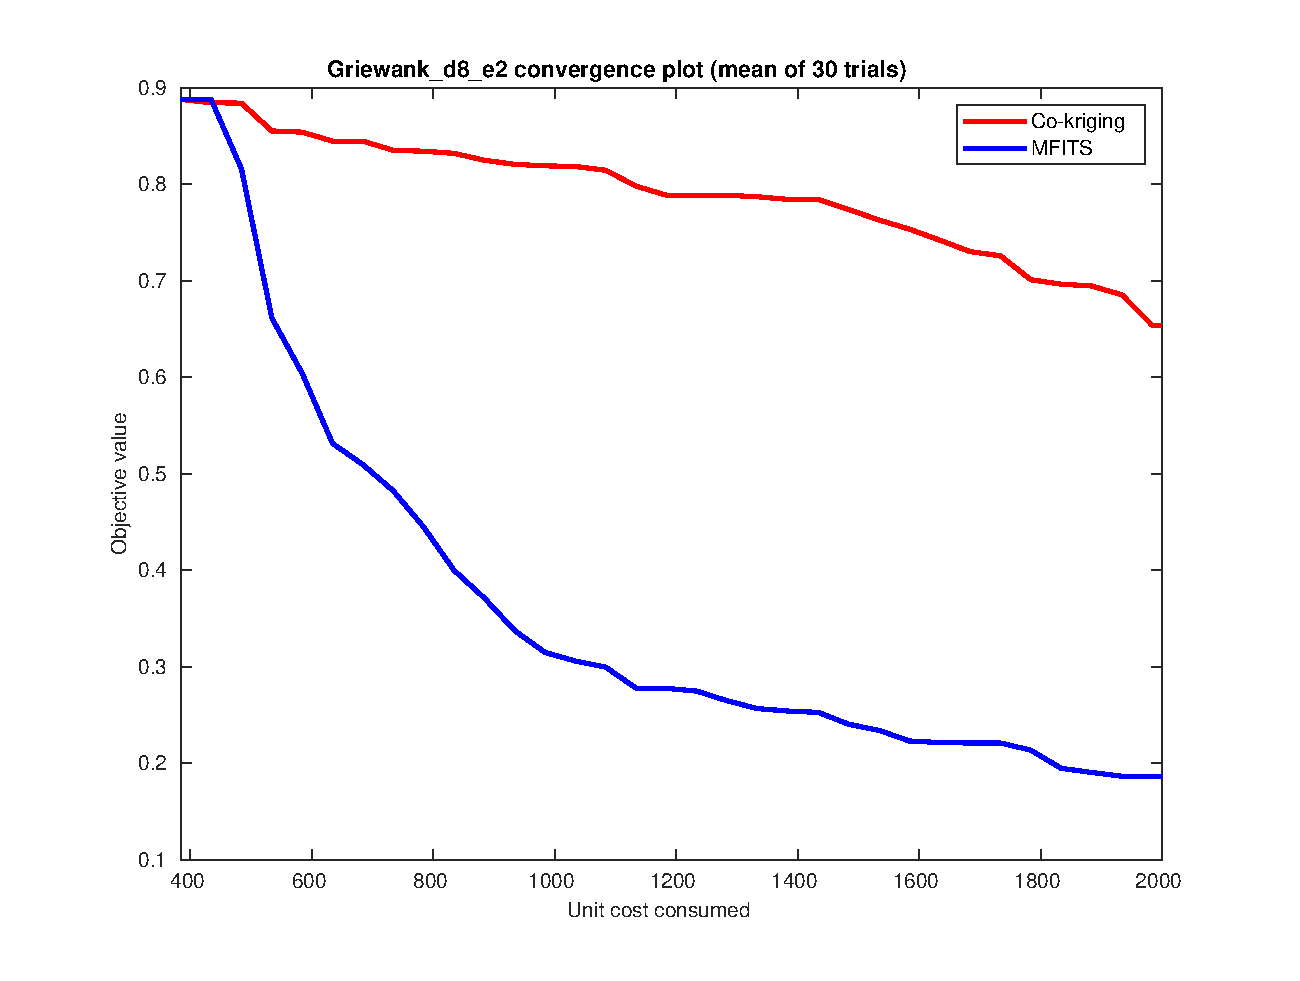
\includegraphics[width = 0.33\textwidth]{img/GW_d8_e2_conv_mean.eps}}\\
  \subfloat[$Griewank_6\ (D=3)$\label{fig:gw63-conv}]{\includegraphics[width = 0.33\textwidth]{img/GW_d3_e6_conv_mean.eps}}
  \subfloat[$Griewank_6\ (D=5)$\label{fig:gw65-conv}]{\includegraphics[width = 0.33\textwidth]{img/GW_d5_e6_conv_mean.eps}}
  \subfloat[$Griewank_6\ (D=8)$\label{fig:gw68-conv}]{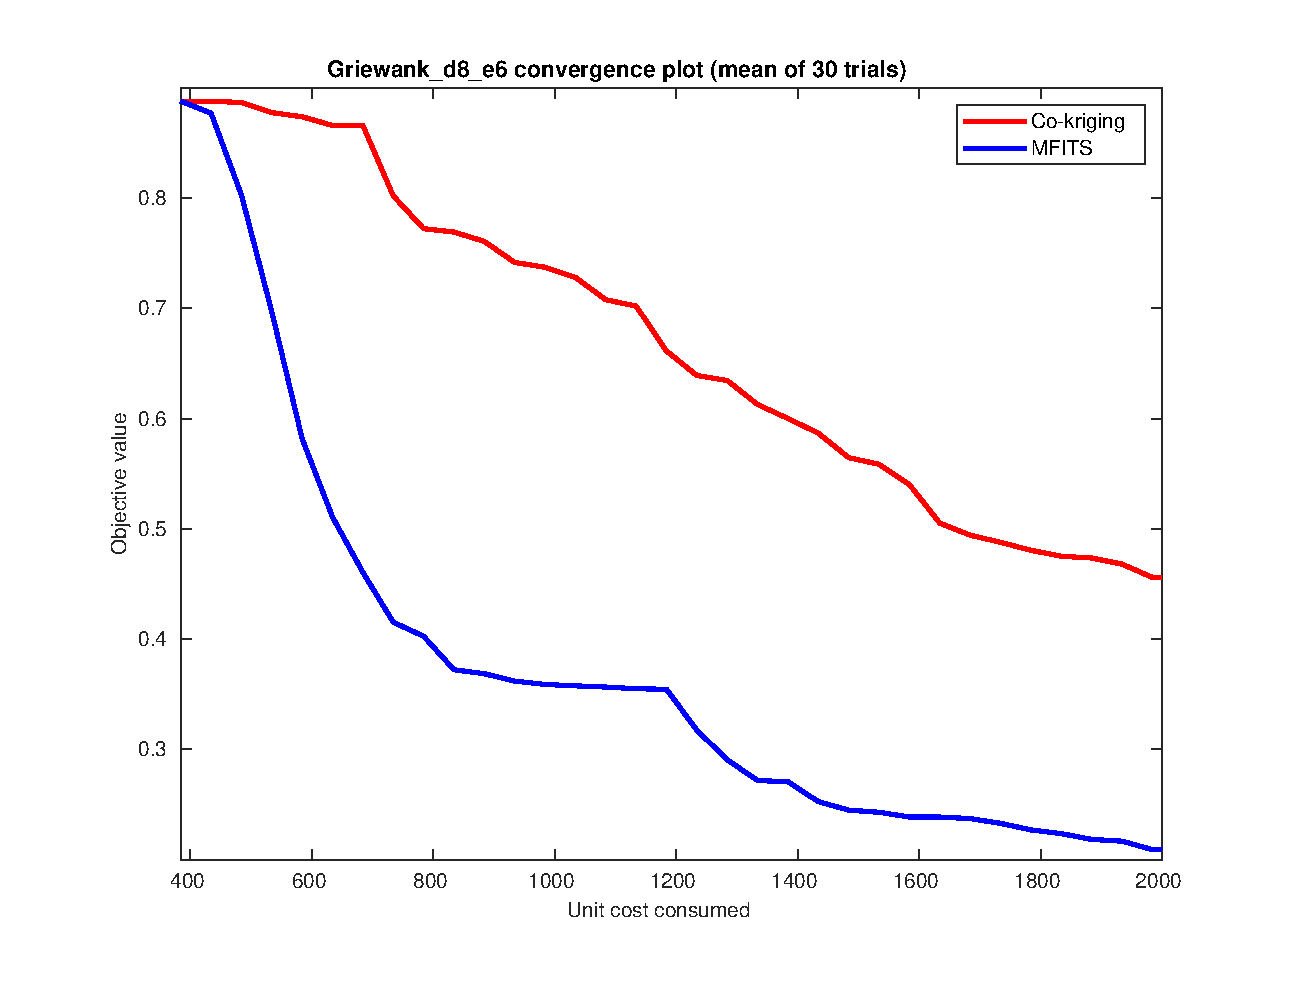
\includegraphics[width = 0.33\textwidth]{img/GW_d8_e6_conv_mean.eps}}
  \caption{Mean convergence plots for $Griewank$ problem instance of dataset $B$, over 30 runs. \angus{will do pgfplots version}} 
    \label{fig:set-b-conv}
\end{figure*}

\subsection*{Summary}
The results from both datasets suggest a similar pattern. For problems with few decision variables, there is very little difference between \AlgName{} and the base-line co-kriging algorithm, and as the size of the problem increases, the convergence rate and performance of \AlgName{} improves over the simple co-kriging algorithm with the greatest improvements being observed on the largest problem instances.

Although both algorithms contain the co-kriging technique as their principal constituent, the base-line algorithm uses a random sampling technique which gives it a disadvantage in problems with more decision variables, as it must cover an exponentially larger space with the same computational budget. By using the $LocalOCBA$ procedure to focus the sampling on areas of the search space that have been identified as promising, \AlgName{} can use its budget more efficently to exploit these regions, which is evidenced by the faster convergence rates at larger problem sizes.

Finally, although the numerical results and convergence plots do indicate that there is not a significant difference between the performance of the two algorithms on the smaller instances; it is worth noting that for three out of four of these instances, the co-kriging baseline did perform slightly better on average. One possible explanation for this is that the $LocalOCBA$ procedure makes \AlgName{} more greedy, and therefore more likely to become trapped in local optima --- especially for multimodal instances like the Griewank problem (as demonstrated in Figure~\ref{fig:grie}). In these smaller instances, the random sampling of the base-line co-kriging algorithm is not as much of a disadvantage and it is more likely to come across good areas of the search space by chance.